\documentclass[12pt]{article}

\usepackage{scicite,times,graphicx,float,hyperref}
\usepackage[skip=0pt]{caption}
\usepackage[utf8]{inputenc}
\usepackage{enumitem}
\usepackage{booktabs}

%%%%%%%%%%%%%%%%%%%%%%%%%%%%%%%%%%%%%%%%%%%%%%%%%%%%%%%%%%%%%%%%%%%%%%%%%%% PREAMBLE %%%%%%%%%%%%%%%%%%%%%%%%%%%%%%%%%%%%%%%%%%%%%%%%%%%%%%%%%%%%%%%%%%%%%%%%%%%

\topmargin -1.0cm
\oddsidemargin 0.0cm 
\textwidth 16cm 
\textheight 23cm
\footskip 1.0cm

\newenvironment{sciabstract}{%
\begin{quote} \bf}
{\end{quote}}

\newcounter{lastnote}
\newenvironment{scilastnote}{%
  \setcounter{lastnote}{\value{enumiv}}%
  \addtocounter{lastnote}{+1}%
  \begin{list}%
  {\arabic{lastnote}.}
  {\setlength{\leftmargin}{.22in}}
  {\setlength{\labelsep}{.5em}}
}
{\end{list}}

\title{Intermediate Report on:\\Pretix Cluster Deployment \& Management} 

\author
{Filipe Pires [85122], João Alegria [85048]\\
\\
Computational Infrastructures Management\\
\normalsize{Department of Electronics, Telecommunications and Informatics}\\
\normalsize{University of Aveiro}\\
} 

\date{\today{}}

%%%%%%%%%%%%%%%%%%%%%%%%%%%%%%%%%%%%%%%%%%%%%%%%%%%%%%%%%%%%%%%%%%%%%%%%%%%% REPORT %%%%%%%%%%%%%%%%%%%%%%%%%%%%%%%%%%%%%%%%%%%%%%%%%%%%%%%%%%%%%%%%%%%%%%%%%%%%

\begin{document} 

\baselineskip18pt

\maketitle 

\section*{Introduction} \label{introduction} %%%%%%%%%%%%%%%%%%%%%%%%%%%%%%%%%%%%%%%%%%%%%%%%%%%%%%%%%%%%%%%%%%%%%%%%%%%%%%%%%%%%%%%%%%%%%%%%%%%%%%%%%%%%%%%%%%%

This report aims to describe the work developed for the intermediate phase of the practical assignment of the discipline of Computational Infrastructures 
Management \cite{assign} from the Msc. degree in Informatics Engineering of the University of Aveiro at the Department of Electronics, Telecommunications and 
Informatics.
It is here included:
a product description and the respective expectations regarding client capacity, derived from a thorough analysis;
the adopted clustering strategy, considering matters such as virtualization, storage, network and load distribution mechanisms;
an explanation of the performance analysis executed based on the department's support platform for representative use cases;
and the results drawn from such analysis, to be considered during the second phase of development.

The service provided is Pretix, an online shop, box office and ticket outlet already successfully used by other service providers for conferences, festivals, 
exhibitions, workshops and more.
All code developed is publicly accessible in our GitHub repository:

\url{https://github.com/FilipePires98/GIC}.

\newpage
\section{Pretix Ticketing Software} \label{pretix} %%%%%%%%%%%%%%%%%%%%%%%%%%%%%%%%%%%%%%%%%%%%%%%%%%%%%%%%%%%%%%%%%%%%%%%%%%%%%%%%%%%%%%%%%%%%%%%%%%%%%%%%%%%%%

% what is pretix?

Pretix \cite{pretix} is an all-in-one product, serving as an online shop, box office and ticket outlet, meant for companies that aim to host events of numerous kinds.
This ticketing software created by Rami.io \cite{rami.io} has a wide variety of features that range from ticket shop customization (domain definition, multiple 
language support, product structure with multiple categories, packages and possibility for donations, seating plans, website embeddings, etc.) and marketing 
(voucher system, email, campaign tracking, etc.), to payment definition (invoicing and multiple payment methods) and on-site management (check-in lists, ticket 
scans, etc.), and even administrative control (with statistics and event-spanning reports, team permissions and data export and API).

As a complete solution, Pretix has already been successfully used for conferences, festivals, concerts, shows, exhibitions, workshops, barcamps, and more 
according to the creators.
The software's source code is completely open source \cite{pretixgit}, and the authors make available extensive documentation \cite{pretixdoc}, an installation 
guide and a support blog.

\subsection{Our Product} \label{pretix.product} %%%%%%%%%%%%%%%%%%%%%%%%%%%%

% what is our purpose? what are we offering?

What we offer, as a developers team, is the Pretix' infrastructure deployment and management as a service that could potentially be provided to businesses 
interested in hosting events by taking advantage of Pretix' many advantages, without having resources or knowledge of how to deploy it themselves.
Our contract is simply to ensure the correct, reliable, secure and constant functioning of Pretix, capable of supporting usage scenarios of the same magnitude 
as of the one described next.

\subsection{Use Case Scenario} \label{pretix.scenario} %%%%%%%%%%%%%%%%%%%%%

% what do we intend to be able to support?
% how many users and/or requests per second is the system supposed to be able to handle?

In order to ensure the fulfillment of our contract, a representative scenario of usage was defined to guide us throughout development.
A simulated organization intends to host a WebSummit-like event by the end of this year.
It has analysed the feature list of Pretix and wishes to adopt it in the future.
However, as it is its first time using the software, the company decided to use it simply as a ticket purchase platform and reduced the payment methods to 
on-site manual payment only. % NUMBERS ? ? ? ? ? ? ? ? ? ? ? ? ? ? ? ? ? ? ? ? ? ? ? ? ? ? ? ? ? ? ? ? ? ? ? ? ? ? ? ? ? ? ? ? ? ? ? ? ? ? ? ? ? ? ? ? ? ? ? ? ?
The organization expects to sell 10 000 tickets in a week and warned us that in previous events they witnessed a peak close to the end of the selling period.

In practical terms this means that we only need to concern ourselves with the online ticket purchasing features and do not even need to consider the actual 
payment process, although it was our intent from the beginning to support most of Pretix's features even if most would not be used.
It also means that we had to build the system considering our hardware limitations and the activity peak expectation.

\subsection{Support Requirements} \label{pretix.requirements} %%%%%%%%%%%%%%

% what components need to exist for the product to be fully supported?
% what are the minimal hardware requirements for its deployment?

As stated in their documentation, to use Pretix it is required:
\vspace{-10pt}
\begin{itemize}[noitemsep]
  \item Pretix and the python packages it depends on
  \item An WSGI application server
  \item A periodic task runner
  \item A database
  \item A reverse proxy
  \item A server for caching, session storage and task queuing
\end{itemize}
\vspace{-10pt}
As we intended to deploy the product in containers, Docker became an additional requirement.

Regarding the hardware remotely available at our department, it was allocated for us an infrastructure of a total of 58 nodes and 115 cores, with 5.6TB of 
storage and 235.8GB of RAM available.
However, this is destined for several developer teams, meaning that we must only use a small portion of such resources, by our estimates of less than 10\% of 
the total capacity.

Also according to Pretix' documentation, the software has some scalability limitations.
In some cases their software needs to "fall back to event-global locking for some actions which are likely to run with high concurrency and cause harm".
For every event, only one of such locking actions can be run at the same time.
With this in mind, they estimate a maximum capacity of approximately 500 orders per minute per event, "even if you add more hardware".
However, they also mention that if the event to be hosted has an unlimited number of tickets (which is our case), fewer locking is applied and thus it is 
possible to reach approximately 1500 orders per minute per event.

Considering all of these aspects, we made an estimation of how many ticket purchase requests we would be able to support per minute.
At this preliminary stage, we believed it could be achieved a capacity of 800 ticket purchases per minute without a relevant amount of failed attempts.
In chapter \ref{performance} we explore our own system in an attempt to determine whether our estimations were correct and feasible or not.

%\texttt{java -cp <userdir>/build/classes fi.FarmInfrastructure}

% \vspace{-10pt}
% \begin{itemize}[noitemsep]
%   \item ...
% \end{itemize}
% \vspace{-10pt}

% \vspace{-10pt}
% \begin{enumerate}[noitemsep]
%   \item ...
% \end{enumerate}
% \vspace{-10pt}

% \begin{figure}[H]
%   \centering
%   \begin{minipage}{\textwidth}
%     \centering
%     \includegraphics[width=\linewidth]{img/.....png}
%   \end{minipage}%
%   \caption{...}
%   \label{...}
% \end{figure} 

\newpage
\section{Clustering Strategy} \label{strategy} %%%%%%%%%%%%%%%%%%%%%%%%%%%%%%%%%%%%%%%%%%%%%%%%%%%%%%%%%%%%%%%%%%%%%%%%%%%%%%%%%%%%%%%%%%%%%%%%%%%%%%%%%%%%%%%%%

\subsection{Architecture} \label{strategy.architecture} %%%%%%%%%%%%%%%%%%%% 

% what are the dependencies? what components does the cluster have?

Docker \cite{docker} allows us to deliver the infrastructure in isolated containers with well-defined communication channels.
This dramatically reduces infrastructure resources required and facilitates its management, while ensuring consistency within the whole environment.
Also, its simplicity in configurations and rapid deployment makes it perfect for its use in any system with a reasonably large size and complexity.

By taking advantage of Pretix' support for Docker, its dependencies were covered after analyzing which technologies would be most appropriate for our scenario.
With an already fully functional Docker Image publicly available \cite{pretix_img}, the authors of the product made the deployment of the web application easier.
In it is the Django-based \cite{django} web application that serves all user interaction, the web server that forwards connections to the application implemented 
with NGinX \cite{nginx} and the Gunicorn \cite{gunicorn} instance supporting the required Web Server Gateway Interface (WSGI).
Pretix' container configuration file also simplified the connection between the product and the storage containers, namely for the required database and caching server.

To handle all storage we chose PostgreSQL \cite{postgresql}.
This relational Database Management System (DBMS) had powerful tools to deal with scalability and redundancy, so it was quickly understood as a good option, 
although others like MariaDB were strongly considered as well.
It is the PostgreSQL that stores the data related to organizations, events, tickets, clients, invoices, etc.
In our case a PostgreSQL cluster is instantiated for redundancy purposes in a Master-Slave mode.
Currently, a single PostgreSQL master and 2 slave nodes are instantiated, and if the master fails the system is capable of assigning one of the slaves as the new master.

A similar approach was followed for the server for caching.
This server has the responsibility of storing in-memory relevant data such as open user sessions, live events, etc. and of asynchronously queuing tasks.
In this case, the chosen tool was Redis \cite{redis}, instantiated in a Master-Slave mode with 1 master and 2 slave nodes as well.
As it is explained in section \ref{strategy.distribution}, the failover process is also supported here.

\subsection{Distribution} \label{strategy.distribution} %%%%%%%%%%%%%%%%%%%%

% how exactly is the system being distributed?

Pgpool \cite{pgpool} was introduced in order to create a robust cluster system and avoid the single point of failure problem.
To do this, 2 pgpool nodes are instantiated and perform lifechecks against nodes to detect faults.
This also allows the load balancing of requests amongst nodes.
As Pgpool can manage multiple PostgreSQL servers, using the replication function it enables the creation of a realtime backup on 2 or more physical disks so 
that the service can continue without stopping servers in case of a disk failure.
Pgpool's connection pooling was also considered a valuable asset in order to reduce connection overhead and improve the system's overall throughput.
Both PostgreSQL and Pgpool have several variations of Docker images available, so we chose 2 whose configurations we found applicable for our purposes 
\cite{postgresql_img} \cite{pgpool_img}.

For Redis, 2 instances of proxies are created to distribute the load of requests and avoid the single point of failure problem.
Once again, Docker Hub contained usable images for both the Redis instances and the proxies \cite{redis_img} \cite{redisproxy_img}.
In this case Redis Sentinel is used to provide a deployment that resists without human intervention certain kinds of failures.
It is the so called sentinels that monitor redis instances and start failover processes when masters are not working as expected to promote a slave replica to 
master and reconfigure the remaining \cite{redis_sentinel}.

But redundancy isn't guaranteed (with its minimum requirements) if other components outside the storage clusters have single points of failure too.
With this in mind, we instantiate 2 Pretix containers, each connected to all Redis proxies and all Pgpool instances.
Additionally, to handle load balancing of requests made to the web servers, we created 2 external proxies using NGinX \cite{nginx_img}. 
These are both connected to both Pretix instances and thus allow the distribution of requests amongst web servers without adding a new single point of failure 
(since if one proxy fails, the other is still capable of forwarding connections to the web servers).

The result is visible in Figure \ref{fig:InfrastructureArchitecture}.

\begin{figure}[H]
  \centering
  \begin{minipage}{.85\textwidth}
    \centering
    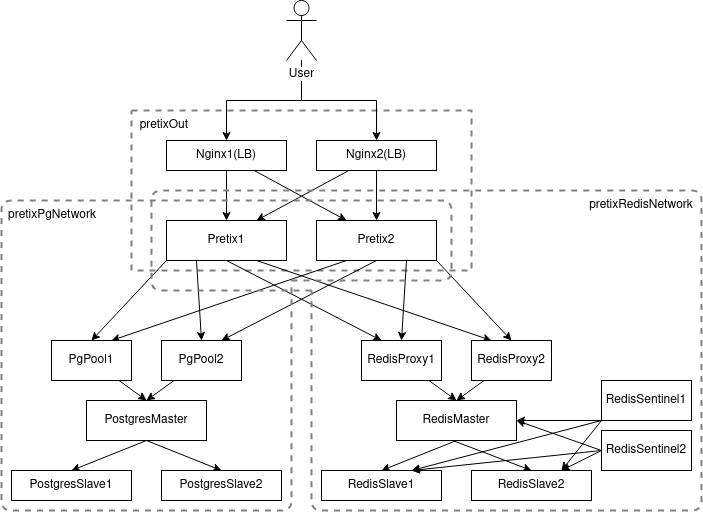
\includegraphics[width=\linewidth]{diagrams/InfrastructureArchitecture.png}
  \end{minipage}%
  \caption{Infrastructure architecture diagram.}
  \label{fig:InfrastructureArchitecture}
\end{figure} 

\subsection{Deployment} \label{strategy.deployment} %%%%%%%%%%%%%%%%%%%%%%%%

% how exactly is the system being deployed?

There are 2 methods of deployment available: either locally or remotely in the department's installations as a docker swarm.
Both alternatives respect the architecture mentioned above but are naturally deployed with some differences in configurations.



...

\newpage
\section{Current Cluster Performance} \label{performance} %%%%%%%%%%%%%%%%%%%%%%%%%%%%%%%%%%%%%%%%%%%%%%%%%%%%%%%%%%%%%%%%%%%%%%%%%%%%%%%%%%%%%%%%%%%%%%%%%%%%%%

% what was done to evaluate its current performance?

In order to determine the true capacity of our deployed solutions, a set of measures were performed both locally and on the remote, shared and more powerful 
infrastructure.
Although replication and redundancy were already concerns of ours, we were not yet focused on determining availability statistics.
Rather, our aim was to test our services in terms of load capacity.

We wished to determine how many users were supported simultaneously accessing Pretix and attempting to purchase tickets to our fictitious event.
To do this, we performed benchmarking tests and tracked the number of failures both in the act of requesting a purchase and in the act of storing purchases in 
our databases.
In this chapter we describe the efforts made for benchmarking and the bottlenecks discovered from our performance evaluation.

\subsection{Benchmarking} \label{performance.benchmarking} %%%%%%%%%%%%%%%%%

% what framework was used for load testing and how was it used?

After doing research on available tools and frameworks, we reached the conclusion that the most adequate would be Locust \cite{locust}.
Locust is an open source, intuitive, distributed, user load testing framework intended to "figure out how many concurrent users a system can handle" by 
programmatically simulating thousands of users called locusts.
During tests, systems are "attacked" by a swarm of locusts whose behavior is defined by the developer in Python and the swarming process is monitored from a 
web UI in real-time. 

When defining the behavior of our locusts, some considerations had to be dealt with.
The job of a locust wasn't simply to send an HTTP request to purchase a ticket; real users need to go through a purchasing process on Pretix' web platform, and 
in that process the user's browser requests far more data from the server than the mere purchase action.
So this process needed to be somehow simulated as well.
Several possibilities were considered to achieve this.

Selenium \cite{selenium}, a suite of tools for automating web browsers, is a widely used solution for testing purposes; however, we intended to launch thousands 
of virtual users and so, even with options such as launching browsers in headless mode (without rendering page elements), this created a bottleneck of processing 
elements that were not relevant to us and did not represent the true capacity of the system, thus rendering the whole benchmark invalid.
Other alternatives like wrappers to drive browsers in Python were tried but proved to be too limited for our purposes.

The solution was to manually go through the purchase process once on the Pretix website and collect all network requests that were being made, including CSS 
resources, image files, Javascript code and requests sent to Pretix' REST API.
Amongst these requests was the actual purchase action in a message of type POST.
Then, we replicated all requests on the locust behavior and, by reading Pretix' API documentation, were able to manipulate the POST request to seem to come 
from different users.
We also included optional data on such requests, like invoices, to increase the load the server needed to process and so establishing a worst-case-scenario usage 
that would give us more comfort regarding the faithfulness of the results.

\subsection{Execution} \label{performance.execution} %%%%%%%%%%%%%%%%%%%%%%%

% how was the benchmarking done?

Having established the behavior of the fictitious users, we proceeded to actually executing our benchmarking.
This was divided in 2 groups of tests of 4 phases each.
The first group was entirely performed locally in one of our personal computers, the second was performed remotely using our Docker Swarm.
This was done in order to clearly comprehend the differences of performance between the 2 deployment methods and detect which bottlenecks were common to both, 
which were surpassed with greater hardware capacity and which appeared only in the second group (if any).

The 4 phases consisted in load testing the solution with 4 different activity peaks: one with half the expected load, one with the expected load, one with 
twice as many expected users and one with 10 times as many users.
These were defined a priori and the expected load was set according to the analysis described in section \ref{pretix.requirements}. \\

The results of the first group of tests are presented next.
... \\



% 400
% 10/s

% ~1 min to 400 simultaneous users
% ~3 min test time

% 9.97 Gb of Mem
% 8 cores at 100\%






With the system fully deployed using Docker Swarm, the second group of tests was executing, resulting in the following values.
... 

\subsection{Bottlenecks} \label{performance.bottlenecks} %%%%%%%%%%%%%%%%%%%

% what performance bottlenecks were found?

...

\newpage
\section{Additional Remarks} \label{remarks} %%%%%%%%%%%%%%%%%%%%%%%%%%%%%%%%%%%%%%%%%%%%%%%%%%%%%%%%%%%%%%%%%%%%%%%%%%%%%%%%%%%%%%%%%%%%%%%%%%%%%%%%%%%%%%%%%%%

\subsection{Pretix Quickstart} \label{remarks.quickstart} %%%%%%%%%%%%%%%%%%

% quickstart script

During development, a need for a faster basic setup of Pretix emerged for debugging purposes.
As many of our tests assumed the existence of organizers and events already inserted on the databases, each time these had to be cleared the objects had to be 
manually created before proceeding with some implementation process.

In order to respond to this need, we developed a Python script capable of completely dispose of the manual labour.
This script, which we called \texttt{quickstart.py} and placed under the scripts folder, uses Selenium \cite{selenium} to create an organization inside Pretix, 
generate a secret API key for sending REST requests (storing it in a text file), create a default event and prepare it for load testing with Locust.
It also contains configurable variables to personalize its output.

Such quickstart tool was not only found useful for the obvious advantage in development speed it brought to us, but was also considered a good help tool for any 
person that wishes to quickly experiment our infrastructure without having to know much about Pretix itself.

\subsection{Planning Phase 2} \label{remarks.planning} %%%%%%%%%%%%%%%%%%%%%

% what is to be done until the final delivery?
% docker secrets, fault tolerance, 

With the intermediate development phase complete, our concerns shift towards making the solution more fault tolerant, scalable, reliable and in general more robust.

...

\subsection{Documentation} \label{remarks.documentation} %%%%%%%%%%%%%%%%%%%

% what documentation was produced?

A great portion of the code we deal with isn't of our authorship, so the documentation it contains is the documentation we get.
Nevertheless, the code we developed has specific purposes and, although usually very much self explanatory due to its nature, should be easy to interpret by any person.
Our goal is to ensure that what we deliver can be easily reused or even continued by other developers.

With this in mind, we made significant efforts on ensuring that all code developed by us followed a common structure with the same coding style.
Also, we made sure all source files have a description of their purpose and relevant information on the first lines, and contain comments on key points of the 
code explaining snippets considered of greater complexity/importance.

\subsection{Assignment Contributions} \label{remarks.contributions} %%%%%%%%

% who did what?

Regarding the work distribution amongst developers, a close-contact strategy was defined where each worked on a cluster component or piece of software according 
to a predefined plan. 
The cluster strategy and respective details were decided in conjunction, as well as the key objectives and tasks to be achieved before the final delivery deadline.

Pretix' features were explored by both developers in order to better comprehend the web platform and the REST API.
Then, João focused on the deployment of our solution on the department's infrastructure while Filipe focused on creating and executing the load tests.
The analysis of the results were carefully conducted in conjunction as well, in order to maintain a common knowledge for better workflows.
It is needless to say that bug and error solving was made along the development phase by both developers any time it was required.

Once performance benchmarking and bottleneck identification were completed, this report and the code documentation became our primary concern, with both 
contributing equally.

\newpage
\section*{Conclusions} \label{conclusions} %%%%%%%%%%%%%%%%%%%%%%%%%%%%%%%%%%%%%%%%%%%%%%%%%%%%%%%%%%%%%%%%%%%%%%%%%%%%%%%%%%%%%%%%%%%%%%%%%%%%%%%%%%%%%%%%%%%%%

...

\begin{thebibliography}{9} %%%%%%%%%%%%%%%%%%%%%%%%%%%%%%%%%%%%%%%%%%%%%%%%%%%%%%%%%%%%%%%%%%%%%%%%%%%%%%%%%%%%%%%%%%%%%%%%%%%%%%%%%%%%%%%%%%%%%%%%%%%%%%%%%%%%%
  \bibliographystyle{Science}

  \bibitem{assign}
    J. P. Barraca,
    \textit{GIC - Report no.1: Simple Product Operation},
    University of Aveiro,
    2019/20.

  \bibitem{pretix}
    \textit{About Pretix},
    \url{https://pretix.eu/about/en/}.
    Pretix.eu,
    retrieved in April 2020.

  \bibitem{rami.io}
    \textit{Welcome to Rami.io},
    \url{https://rami.io/}.
    Rami.io,
    retrieved in April 2020.

  \bibitem{pretixgit}
    \textit{Pretix Code Repository},
    \url{https://github.com/pretix/pretix}.
    GuitHub, Inc.,
    retrieved in April 2020.

  \bibitem{pretixdoc}
    \textit{Welcome to pretix' documentation!},
    \url{https://docs.pretix.eu/en/latest/}.
    Pretix.eu,
    retrieved in April 2020.



  \bibitem{locust}
    \textit{Locust, an open source load testing tool},
    \url{https://locust.io/}.
    Locust.io,
    retrieved in April 2020.

  \bibitem{selenium}
    \textit{About Selenium},
    \url{https://www.selenium.dev/about/}.
    Software Freedom Conservancy,
    retrieved in April 2020.

\end{thebibliography}

\clearpage

\end{document}




















